%%%%%%%%%%%%%%%%%%%%%%%%%%%%%%%%%%%%%%%%%%%%%%%%%%%%%%%%%%%%%%%%%%%%%%%%%%%%%%%%
%%%%%%%%%%%%%%%%%%   Vorlage für eine Abschlussarbeit   %%%%%%%%%%%%%%%%%%%%%%%%
%%%%%%%%%%%%%%%%%%%%%%%%%%%%%%%%%%%%%%%%%%%%%%%%%%%%%%%%%%%%%%%%%%%%%%%%%%%%%%%%

% Erstellt von Maximilian Nöthe, <maximilian.noethe@tu-dortmund.de>
% ausgelegt für lualatex und Biblatex mit biber

% Kompilieren mit 
% latexmk --lualatex --output-directory=build thesis.tex
% oder einfach mit:
% make

\documentclass[
  tucolor,       % remove for less green,
  BCOR=12mm,     % 12mm binding corrections, adjust to fit your binding
  parskip=half,  % new paragraphs start with half line vertical space
  open=any,      % chapters start on both odd and even pages
  cleardoublepage=plain,  % no header/footer on blank pages
]{tudothesis}


% Warning, if another latex run is needed
\usepackage[aux]{rerunfilecheck}

% just list chapters and sections in the toc, not subsections or smaller
\setcounter{tocdepth}{1}

%------------------------------------------------------------------------------
%------------------------------ Fonts, Unicode, Language ----------------------
%------------------------------------------------------------------------------
\usepackage{fontspec}
\defaultfontfeatures{Ligatures=TeX}  % -- becomes en-dash etc.

% german language
\usepackage{polyglossia}
\setdefaultlanguage{german}

% for english abstract and english titles in the toc
\setotherlanguages{english}

% intelligent quotation marks, language and nesting sensitive
\usepackage[autostyle]{csquotes}

% microtypographical features, makes the text look nicer on the small scale
\usepackage{microtype}

%------------------------------------------------------------------------------
%------------------------ Math Packages and settings --------------------------
%------------------------------------------------------------------------------

\usepackage{amsmath}
\usepackage{amssymb}
\usepackage{mathtools}

% Enable Unicode-Math and follow the ISO-Standards for typesetting math
\usepackage[
  math-style=ISO,
  bold-style=ISO,
  sans-style=italic,
  nabla=upright,
  partial=upright,
]{unicode-math}
\setmathfont{Latin Modern Math}

% nice, small fracs for the text with \sfrac{}{}
\usepackage{xfrac}

%------------------------------------------------------------------------------
%---------------------------- Numbers and Units -------------------------------
%------------------------------------------------------------------------------

\usepackage[
  locale=DE,
  separate-uncertainty=true,
  per-mode=symbol-or-fraction,
]{siunitx}
\sisetup{math-micro=\text{µ},text-micro=µ}

%------------------------------------------------------------------------------
%-------------------------------- tables  -------------------------------------
%------------------------------------------------------------------------------

\usepackage{booktabs}       % \toprule, \midrule, \bottomrule, etc

%------------------------------------------------------------------------------
%-------------------------------- graphics -------------------------------------
%------------------------------------------------------------------------------

\usepackage{graphicx}
% currently broken
% \usepackage{grffile}

% allow figures to be placed in the running text by default:
\usepackage{scrhack}
\usepackage{float}
\floatplacement{figure}{htbp}
\floatplacement{table}{htbp}

% keep figures and tables in the section
\usepackage[section, below]{placeins}


%------------------------------------------------------------------------------
%---------------------- customize list environments ---------------------------
%------------------------------------------------------------------------------

\usepackage{enumitem}

%------------------------------------------------------------------------------
%------------------------------ Bibliographie ---------------------------------
%------------------------------------------------------------------------------

\usepackage[
  backend=biber,   % use modern biber backend
  autolang=hyphen, % load hyphenation rules for if language of bibentry is not
                   % german, has to be loaded with \setotherlanguages
                   % in the references.bib use langid={en} for english sources
]{biblatex}
\addbibresource{references.bib}  % the bib file to use
\DefineBibliographyStrings{german}{andothers = {{et\,al\adddot}}}  % replace u.a. with et al.


% Last packages, do not change order or insert new packages after these ones
\usepackage[pdfusetitle, unicode, linkbordercolor=tugreen]{hyperref}
\hypersetup{
	pdfusetitle,
	unicode,
	colorlinks,
	linkcolor={tugreen},
	citecolor={tugreen},
	urlcolor={tugreen}
}

\usepackage{bookmark}
\usepackage[shortcuts]{extdash}

%------------------------------------------------------------------------------
%-------------------------    Angaben zur Arbeit   ----------------------------
%------------------------------------------------------------------------------

\author{Benjamin Matthias Biehler}
\title{Graphisch-interaktive Entwicklungsumgebung für Robotersysteme zum Einsatz in den Rehabilitationswissenschaften}
\date{2021}
\birthplace{Nürnberg}
\chair{Lehrstuhl für Computergraphik VII}
\division{Fakultät Informatik}
\thesisclass{Bachelor of Science}
\submissiondate{31. September 2021}			% TODO Abgabedatum
\firstcorrector{PD~Dr.~Weichert}
\secondcorrector{Prof.~Dr.-Ing.~Bühler}

% tu logo on top of the titlepage
\titlehead{
\includegraphics[height=1.5cm]{logos/tu-logo.pdf}}

\begin{document}
\frontmatter
\maketitle

% Gutachterseite
\makecorrectorpage

% hier beginnt der Vorspann, nummeriert in römischen Zahlen
\thispagestyle{plain}

\section*{Kurzfassung}
Hier steht eine Kurzfassung der Arbeit in deutscher Sprache inklusive der Zusammenfassung der
Ergebnisse.
Zusammen mit der englischen Zusammenfassung muss sie auf diese Seite passen.

\section*{Abstract}
\begin{english}
The abstract is a short summary of the thesis in English, together with the German summary it has to fit on this page.
\end{english}

\tableofcontents

\mainmatter
% Hier beginnt der Inhalt mit Seite 1 in arabischen Ziffern
\chapter{Einleitung}
Hier folgt eine kurze Einleitung in die Thematik der Bachelorarbeit.
Die Einleitung muss kurz sein, damit die vorgegebene Gesamtlänge der 
Arbeit von 25 Seiten nicht überschritten wird. 
Die Beschränkung der Seitenzahl sollte man ernst nehmen,
da Überschreitung zu Abzügen in der Note führen kann. 
Um der Längenbeschränkung zu genügen, darf auch nicht an der Schriftgröße,
dem Zeilenabstand oder dem Satzspiegel (bedruckte Fläche der Seite) manipuliert werden.
 		
\chapter{Mensch-Roboter-Interaktion} %TODO

\section{Herausforderungen} %TODO
Was sind die Probleme, die mit der Anwendung gelöst werden sollen? Was waren die Hindernisse, die sich für diese Arbeit gestellt haben? 

\section{Stand der Technik} %TODO
Werden ähnliche Tools bereits eingesetzt, wenn ja mit welchem Erfolg? Was war der bisherige Ansatz in dieser Domäne (Pepper-Programmierung)?

\section{Kollaborations-Schnittstelle} %TODO
Was ergibt sich aus 2.1 und 2.2 für die Arbeit? Welche grobe Zielsetzung wurde festgelegt?





\begin{figure} %TODO Löschen, wenn erstes Bild eingefügt
	\centering
	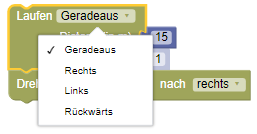
\includegraphics[width=5cm]{Plots/zz-placeholder.png}
	\caption{Platzhalter für Abbildungsverzeichnis.}
	\label{fig:placeholder}
\end{figure}		
\chapter{Interaktive Visuelle Robotersteuerung}\label{ch:interak-vis-roboterst} %TODO
1-2 Absätze die dieses Kapitel einleiten (wahrscheinlich längstes Kapitel der Arbeit).

Beschreibung des GUIs und der Prinzipien dahinter. Unterkapitel gerne nochmal durchmischen.

\section{Endbenutzer-Entwicklung} %TODO umbenennen
% Was ist Endbenutzer-Entwicklung/EUD? Was sind die Anwendungsbereiche? Welche Probleme können sie darstellen? 
Damit die Robotersteuerung durch Endbenutzer ermöglicht werden kann muss die Entwicklungsumgebung Endbenutzer-Entwicklung umsetzen. Dies ist ein aktueller Forschungszweig, der sich mit Methoden, Techniken und Werkzeugen beschäftigt, die Endbenutzern anstelle von professionellen Software-Entwicklern die Anpassung, Erweiterung oder Entwicklung von Software ermöglichen \cite{Lieberman2006EUDaEP}.

Da es, wie in Kapitel \ref{sec:2.3-kollab} beschrieben, das Ziel der Entwicklungsumgebung war, Endbenutzern die Möglichkeit zu geben eigenständig ebendiese Aufgaben zu erfüllen ist es wichtig die verbreiteten Ansätze dieses Forschungsfeldes zu betrachten.

Endbenutzer-Entwicklung beschäftigt sich mit einem breiten Feld von verschiedenen Anwendungsfällen. Diese reichen von Tabellenkalkulation, über mobile Anwendungen und Websiten, bis hin zu der Programmierung von industriellen Robotern. Diese verschiedenen Domänen ziehen ebenso verschiedene Lösungsansätze mit sich. Im folgenden werden mehrere dieser Ansätze kurz eingeführt, mit denen Roboterprogrammierung ermöglicht werden könnte. Daraufhin wird erklärt welcher dieser Ansätze genutzt wurde um die Entwicklungsumgebung umzusetzen, und wieso dieser den anderen vorgezogen wurde. %TODO Cite Domänen

%\hspace{0.5cm}
%\hrule
%
%Endbenutzer-Entwicklung ist, nach \citeauthor{Lieberman2006EUDaEP} \cite{Lieberman2006EUDaEP}, ein aktuelles Forschungsgebiet der Mensch-Maschine-Interaktion, das sich damit beschäftigt Methoden, Techniken und Werkzeuge zu entwickeln, die es Endnutzern, anstelle von professionellen Software-Entwicklern, ermöglichen in irgendeiner Weise Teile von Software anzupassen, erweitern oder sogar eigenständig zu entwickeln.
%
%Die Domäne der Endbenutzer-Entwicklung erstreckt sich von der Automatisierung von Tabellen in Tabellenkalkulations-Programmen und einfachen Makros in Textbearbeitungsprogrammen \cite{Scaffidi2005EstimatingNEUP}, über mobile Anwendungen \cite{Wolber2011AppInventor} oder Webseiten \cite{Rode2005EUDWebDev}, bis hin zu der Entwicklung von kritischen Anwendungen im Gesundheitssystem \cite{Lindgren2010ModelPKSHD}. Aktuelle Schätzungen in den USA zufolge arbeiten 90 Millionen Endbenutzer mit einer Form von Endbenutzer-Entwicklung, während nur 3 Millionen professionelle Programmierer dort arbeiten \cite{Scaffidi2005EstimatingNEUP}. \colorbox{yellow}{aktuellere Daten?}
%
%Diese Weise Software zu entwickeln bringt jedoch auch viele Probleme, wie etwa Sicherheitslücken, mit sich \cite{Harrison2004DangersEUP}. Um diese und andere kritische Fehler, die in der Programmierung der jeweiligen Anwendungen vorkommen können, zu verhindern muss die EUD-Programmierumgebung die Sicherheit und Korrektheit der entstehenden Software sicher stellen, und mögliche Fehler des Endbenutzers finden oder korrigieren können. Bei der Entwicklung von Anwendungen für soziale Roboter sind Sicherheitsbedenken weniger relevant, da die Roboter nicht auf Daten arbeiten, die von kritischer Bedeutung sind und das mögliche Verhalten der Roboter klar definiert ist.

\subsection{Arten von Endbenutzer-Entwicklung}
% Welche Arten von EUD gibt es? Wie unterscheiden sich die Ansätze zum Ermöglichen von EUD? Was ist No-Code, Low-Code, Macro-Programmierung, Programming by Example etc.? 
Low-Code Plattformen verringern, meistens durch graphische Benutzerschnittstellen, den Bedarf an von Hand geschriebenen Code. Je nach Plattform müssen jedoch einige Teile von Anwendungen noch selbst geschrieben werden. Dies vereinfacht und beschleunigt die Entwicklung für professionelle Programmierer und senkt die Barriere für Endbenutzer . Im Falle von No-Code Plattformen entfällt der Bedarf Code zu schreiben komplett und macht es Endbenutzern möglich diese Plattformen eigenständig zu benutzen. Diese Plattformen nutzen meist einen graphischen Ansatz, um die Programmierung ohne Code zu ermöglichen, und sind mit dem Begriff der Visuellen Programmierung verwandt. % TODO zitieren

Natural Language Programming ist der Ansatz, dass Endbenutzer Programme in normalen deutschen oder englischen Sätzen schreiben. Die Sätze und Programm-Dateien folgen dabei trotzdem noch einer klar definierten Struktur, um die Interpretation durch den Computer zu ermöglichen. Aus den so geschriebenen Dateien generiert die Programmierumgebung dann für die Maschine lesbaren Code \cite{Nadkarni2011NLPIntroduction}.

Programming By Example - bei der Anwendung mit Robotern auch Programming By Demonstration genannt - versucht es zu ermöglichen, dass der Endbenutzer dem Roboter oder Computer vorführt was dieser tun soll. Dies kann entweder durch Datenpaare von Ein- und Ausgabe \cite{Singh2015PredictionPBE} oder durch Sensoren geschehen, die beispielsweise Robotern gewünschte Bewegung vorführen. Daraus kann sich dann ein Anlern-Prozess entwickeln, in dem die Maschine selbst Beispiele ausführt, deren Fehler der Endbenutzer dann korrigieren kann \cite{Kurlander1993WatchPBD}.

\colorbox{yellow}{Evtl. weitere Konzepte kurz umreißen}

\subsection{Auswahl des Enbenutzer-Entwicklungs Konzepts}

Um die Entwicklungsumgebung zu erstellen wurde die Entscheidung getroffen eine No-Code Plattform zu nutzen. Einerseits sind sowohl Programming By Demonstration, als auch Natural Language Programming weitaus komplexer zu realisieren, als visuelle No-Code Plattformen. Weiterhin sind Natural Language Programming Ansätze eher auf textbasierte Anwendungen, wie maschinelle Übersetzungen und Informationsauswertung, optimiert \cite{Liddy2001NLP}. Dagegen sind visuelle No-Code Plattformen auf prozedurale Programmierung spezialisiert und mit Hilfe von einfachen Bibliotheken leicht zu realisieren. Auch sind visuell dargestellte Programme leichter zu verstehen als Textbasierte und bieten mehr Überblick über den Ablauf des Programmes. %TODO studies finden

\colorbox{yellow}{Weiter ausführen. Studien lesen.}

%Vorteile No-Code: Überblick, Anpassung, Einfachheit

\section{Visuelle Programmierung} \label{sec:visuelle-programmierung} %TODO umbenennen
%Was ist Visuelle Programmierung? Wozu ist sie sinnvoll nutzbar? Was sind Schwächen und Herausforderungen bei der Entwicklung einer solchen Schnittstelle?

Visuelle Programmierung ersetzt die textuellen Elemente traditioneller Programmiersprachen ausschließlich durch graphische Bausteine \cite{Schiffer1996VisuelleProgPG}. Historisch gesehen werden sie besonders in pädagogischen Umfeld \cite{SaezLopez2016VPLElementarySchool}, Benutzeroberflächen \cite{Rode2005EUDWebDev} und Robotik \cite{Weintrop2018CoBloxRoboticsProg} und sind meist dazu ausgelegt von nicht professionellen Endbenutzern bedienbar zu sein.

Dementsprechend eignet sich ein visueller Programmieransatz für die Realisierung der Entwicklungsumgebung für Pepper.

\colorbox{yellow}{23.8.}

\subsection{Visuelle Programmierung in der Robotik}

\subsection{Eigenschaften von Visueller Programmierung}
% Wie ist VP definiert? Welche Arten von VP gibt es? 

\subsection{Block-Programmierung} 
% Wie funktionieren Block-Basierte Programmiersprachen? Wieso werden sie häufig im EUD-Kontext eingesetzt? Welche Probleme stellen sich bei der Programmierung in Block-Sprachen? Was ist Blockly?

\section{Iterativer Entwicklungszyklus} \label{sec:iterative-entwicklung} %TODO			
\chapter{Roboter-Ansteuerung}\label{ch:roboter-steuerung} %TODO
% GROßES TODO:
% Überschriften anpassen
% Inhalte abgleichen

\section{Sprachausgabe}


\section{Bewegungssteuerung} %TODO


\section{Spracherkennung} %TODO
		
\chapter{Benutzerzentrierte Realisierung}\label{ch:benutzerzentrierte-realisierung} %TODO
Damit die Realisierung der graphisch-interaktiven Entwicklungsumgebung auf die Nutzenden angepasst werden kann, wurden die Vorlieben der Nutzenden mit verschiedenen Methoden abgefragt. Die daraus entstandenen Ergebnisse wurden bei der Entwicklung berücksichtigt. Das folgende Kapitel führt die beiden Konzepte ein und erklärt, wie diese angewendet wurden.

In Abschnitt \ref{sec:anforderungserhebung} wird das Konzept des Fragebogens erläutert, mit dem die Anforderungen der Nutzenden erhoben wurden. Daraufhin wird in Abschnitt \ref{sec:testsettings} die Struktur der teilnehmenden Beobachtung aufgeführt, mit der das Feedback der Nutzenden gesammelt wurde. Zuletzt wird in Abschnitt \ref{sec:operationalisierung} die Anwendung dieser beiden Konzepte und die Rekrutierung der Nutzenden dargelegt.

\section{Gestaltung der Anforderungserhebung}\label{sec:anforderungserhebung}
% Wie wurden anfänglich die Anforderungen der Nutzer erhoben?

Um die Entwicklungsumgebung auf die Bedürfnisse der Nutzenden anzupassen, müssen deren Anforderungen abgefragt werden. Zu diesem Zweck bietet sich besonders durch die Möglichkeit der Einbindung von zusätzlichen Medien eine gezielte Online-Befragung an \cite{Schnell2018MethodenES}. Aus den Ergebnissen dieser Befragung entstand dann ein anfänglicher Style-Guide für die Benutzeroberfläche.

Damit die Befragung nützliche Ergebnisse liefert, müssen alle Fragen verständlich, knapp und neutral formuliert sein \cite{Jacobsen2019PraxisbuchUuU}. Der Fragebogen wurde in einzelne Abschnitte unterteilt, die alle nötigen Informationen enthielten und ohne Scrollen angezeigt werden konnten. Um technischen Problemen, die durch verschiedene Endgeräte und Browser entstehen könnten \cite{Schnell2018MethodenES}, vorzubeugen, wurde die Online-Umfrage-Applikation LimeSurvey verwendet. Diese bot alle nötigen Funktionen wie die Möglichkeit, Teilnehmende an der Umfrage zu verwalten und die Daten in der Anwendung auszuwerten. %und wurde bereitgestellt? Zitieren?

Bevor den Teilnehmenden an der Umfrage Fragen gestellt wurden, wurde Pepper, siehe Kapitel \ref{ch:roboter-steuerung}, und das Anwendungsbeispiel in Abbildung \ref{fig:umfrage-anwendungsbeispiel} vorgestellt und erklärt. Das Anwendungsbeispiel, das die Umfrage begleitet, besteht nur daraus, dass Pepper sich vorstellt und dann das Gegenüber fragt, ob Pepper sich bewegen oder eine Geschichte erzählen soll. Sagt die Person "Bewegen" oder "Geschichte", führt Pepper die gewünschte Aktion aus.

\begin{figure}[t]
	\centering
	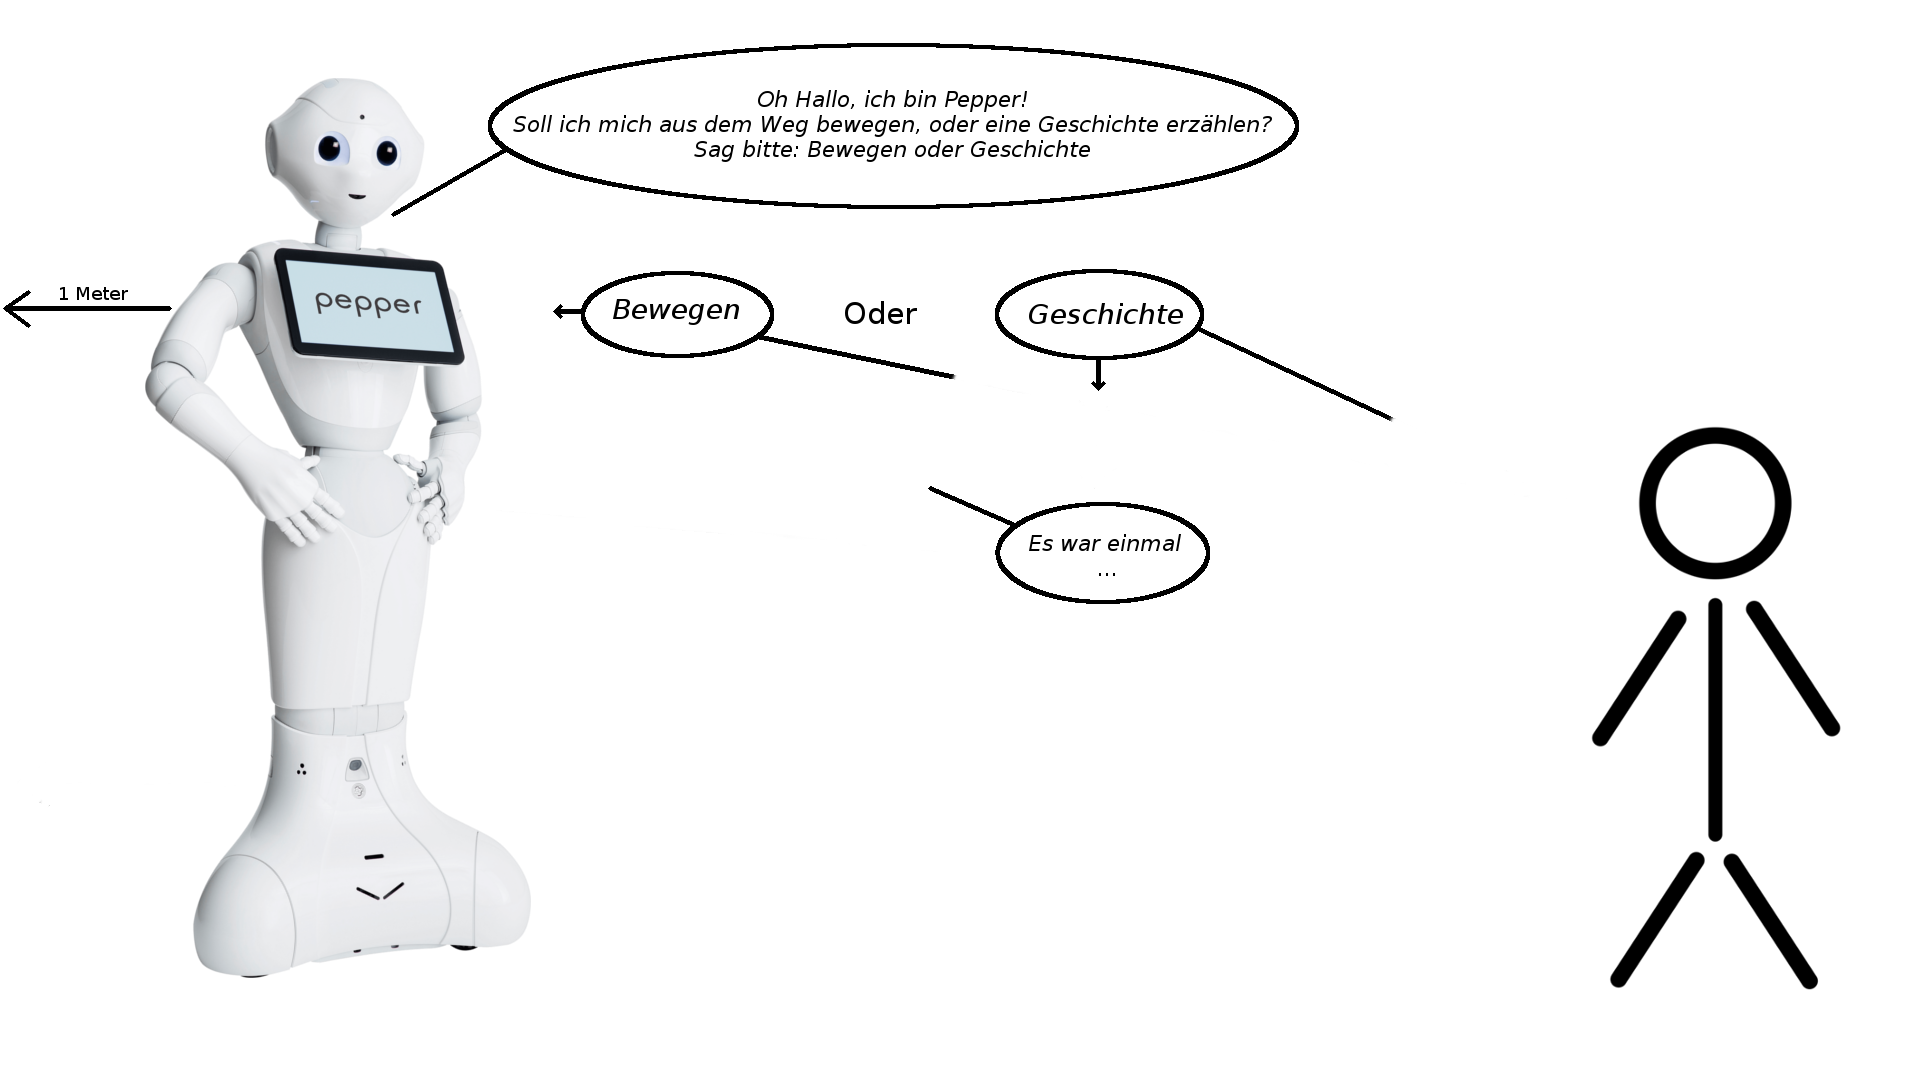
\includegraphics[width=13cm]{Plots/umfrage-anwendungsbeispiel.png}
	\caption{Anwendungsbeispiel der Anforderungserhebung.}
	\label{fig:umfrage-anwendungsbeispiel}
\end{figure}


In den folgenden Abschnitten werden die einzelnen Teile des Fragebogens und deren Nutzen für den Entwicklungsprozess aufgeführt. Die Auswertung der Ergebnisse des Fragebogens folgt in Kapitel \ref{sec:quanti-auswertung}.

\subsection{Vergleich mit bestehenden Anwendungen}
Der erste Anschnitt der Umfrage stellt Choregraphe, siehe Abschnitt \ref{sec:stand-der-technik}, und das Konzept der Entwicklungsumgebung mithilfe eines Mock-ups vor. Dabei werden die grundlegenden Funktionen beider Programme erläutert. Dazu wird jeweils die Realisierung des Anwendungsbeispiels aus Abbildung \ref{fig:umfrage-anwendungsbeispiel} in beiden Entwicklungsumgebungen, siehe Abbildung \ref{fig:umfrage-anwendung}, dargestellt.

\begin{figure}[t]
	\centering
	\begin{subfigure}{.5\textwidth}
		\centering
		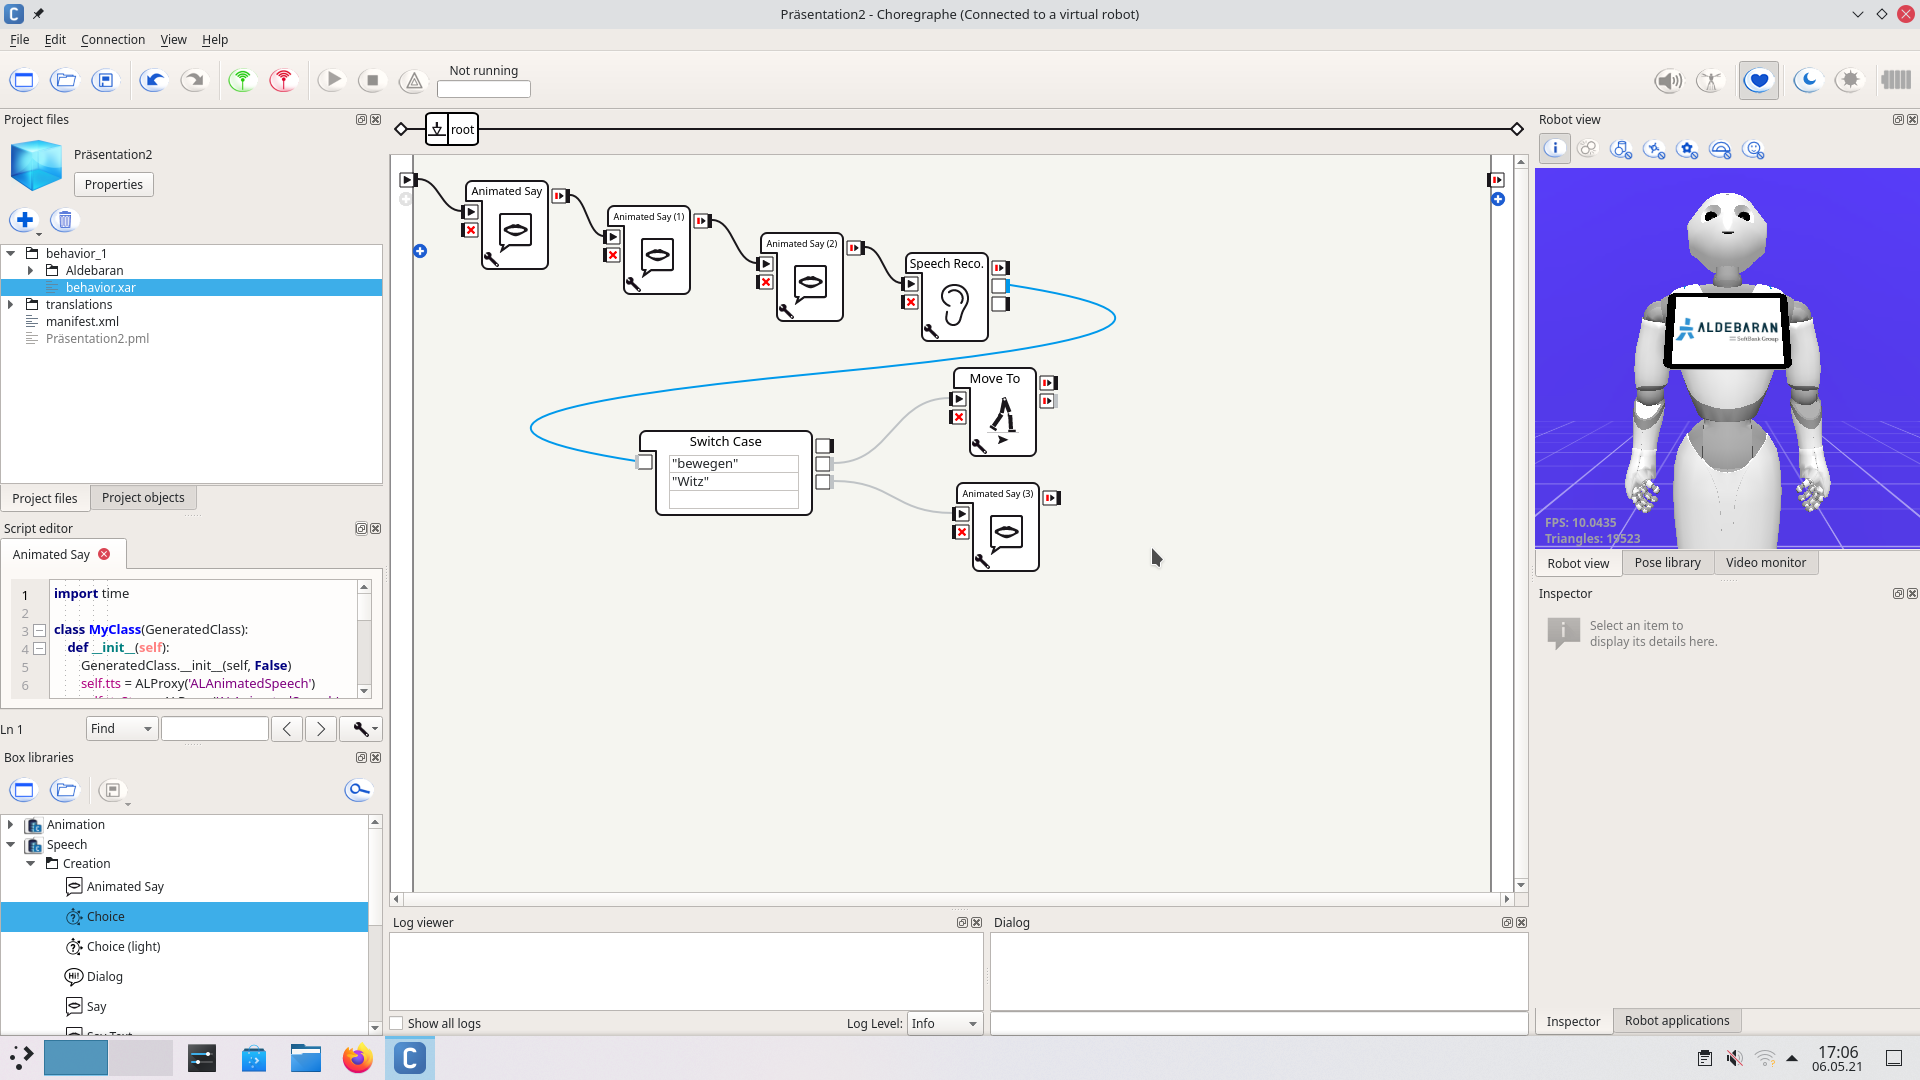
\includegraphics[width=\linewidth]{Plots/umfrage-choregraphe-anwendung.png}
		\caption{Anwendung in Choregraphe.}
		\label{subfig:choregraphe-anwendung}
	\end{subfigure}%
	\begin{subfigure}{.5\textwidth}
		\centering
		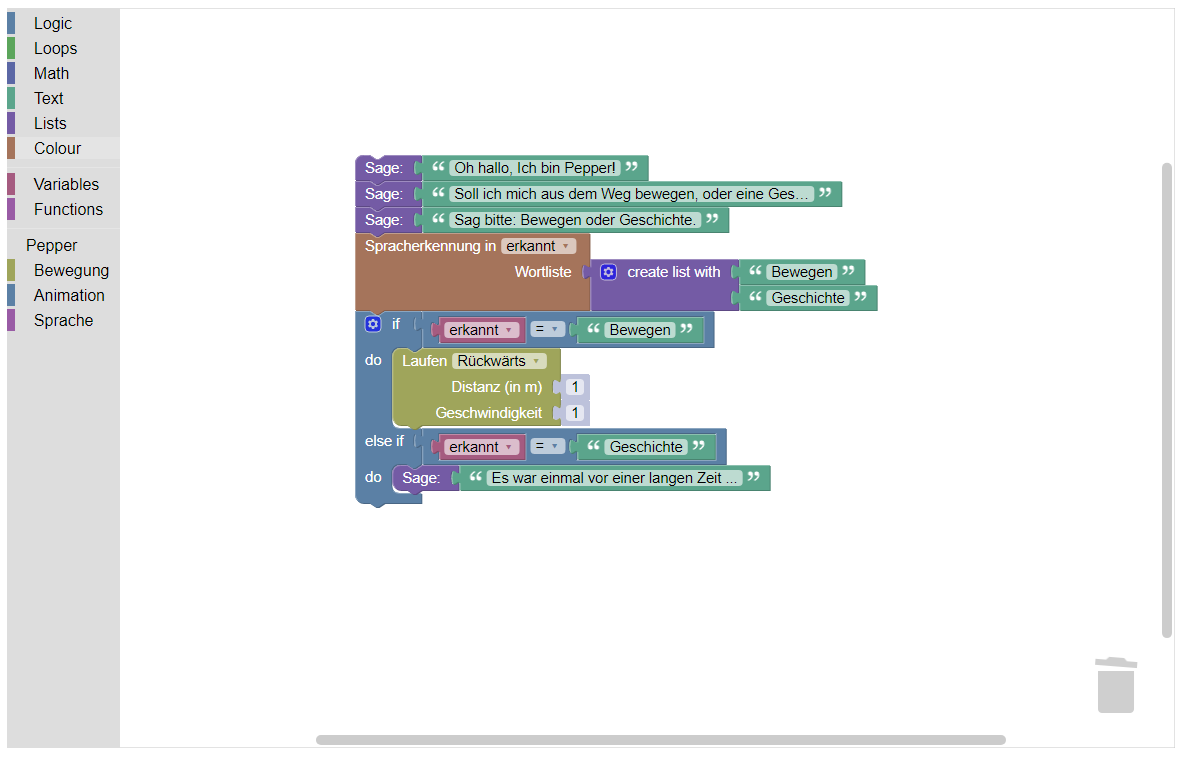
\includegraphics[width=\linewidth]{Plots/umfrage-blockly-anwendung.png}
		\caption{Anwendung im Blockly Mock-up.}
		\label{subfig:blockly-anwendung}
	\end{subfigure}
	\caption{Das Anwendungsbeispiel in Choregraphe und dem Blockly Mock-up umgesetzt.}
	\label{fig:umfrage-anwendung}
\end{figure}

Die Teilnehmenden an der Umfrage werden daraufhin aufgefordert, neun Aussagen auf je einer Skala für beide Entwicklungsumgebungen zu bewerten. Zu diesem Zweck wurde eine 5-Punkte Likert-Skala \cite{Schnell2018MethodenES} verwendet, die eine neutrale Antwortmöglichkeit zulässt. Diese sollte existieren, damit die Teilnehmenden nicht gezwungen sind, eine Entscheidung zu treffen \cite{Willits2016AnotherLookLikert}, falls sie wegen ihrer fehlenden Erfahrung unsicher sind. Die beiden Extrema der Skala sind mit "1: Stimme überhaupt nicht zu" und "5: Stimme voll zu" beschriftet. Diese Skala wird im weiteren Verlauf des Fragebogens weiterhin verwendet, um Konsistenz zu schaffen.

Die Aussagen beziehen sich insbesondere auf Verständlichkeit der Benutzeroberfläche, Einschätzung der eigenen Fähigkeit, die Entwicklungsumgebung zu nutzten und Interesse an der Nutzung der Anwendungen. %TODO Direkt die Aussagen hier einbinden? -> 121321311 (1 Verst., 2 Eisch., 3 Int.)

Die hier erhobenen Daten wurden dazu genutzt, eine erste Einschätzung des Mock-ups zu erlangen. Außerdem gaben sie eine Indikation, ob ein direkter Vergleich der beiden Entwicklungsumgebungen in den Nutzertests nötig ist.

\subsection{Blockgestaltung}
\colorbox{red}{Weiter, Übergänge dazwischen finden}

Wie bereits in Kapitel \ref{sec:visuelle-programmierung} dargelegt, gibt es verschiedene Möglichkeiten Blöcke in Blockly zu gestalten. Um diese Designentscheidungen den Nutzenden anzupassen, werden im zweiten Abschnitt der Online-Umfrage den Teilnehmenden jeweils verschiedene Mock-ups von funktional gleichen Blöcken präsentiert. Sie sollen dann den für sie am einfachsten verständlichen Block auswählen.

Die Auswahl der verschiedenen Optionen wurde so gewählt, dass die Mock-ups, die zur Auswahl stehen, jeweils Designentscheidungen repräsentieren. Beispielsweise steht die Entscheidung in Abbildung \textbf{TODO} repräsentativ für die Option einzelne Blöcke mit Hilfe von Drop-Down-Menüs zusammenzufassen und die Entscheidung Parameter-Slots generell extern (rechts) oder intern (mitten im Block) bereitzustellen. %TODO Zusammenschneiden der Designentscheidung 

Die gesammelten Antworten werden in den Style-Guide übersetzt, der die Vorlieben der Teilnehmenden an der Umfrage repräsentiert.

\subsection{Funktionale Anforderungen}
Im darauf folgenden Abschnitt des Fragebogens werden konkrete Anforderungen abgefragt. Den Teilnehmenden werden verschiedene Aussagen präsentiert, die sie auf einer 5-Punkte Likert-Skala bewerten sollen. Da die Teilnehmenden bereits eine Einführung in die Entwicklungsumgebung erhalten haben und sie im vorangegangenen Abschnitt des Fragebogens verschiedene Mock-ups und Kontrollelemente kennengelernt haben, haben sie nun ein Verständnis der Benutzeroberfläche um diese Anforderungen zu bewerten. %TODO etwas schöner formulieren?

Die abgefragten Anforderungen bezogen sich auf Barrierefreiheit, Sprache der Benutzeroberfläche, integrierte Funktionen in der Oberfläche, Benutzungsweise der Entwicklungsumgebung und weitere Funktionen dieser.

Teile dieser Anforderungen, wie die Sprache und Benutzungsweise der Benutzeroberfläche, flossen ebenso in den Style-Guide, siehe \ref{app:style-guide}, ein. Weitere Teile dieser Ergebnisse, wie etwa die Aussagen zu Barrierefreiheit, Erklärungen und Funktionen in der Benutzeroberfläche, bildeten eine Prioritäten-Liste von Funktionen, die in diese Anwendung eingefügt werden können.

%Eine weitere wichtige Komponente des Fragebogens ist die Abfrage der Anforderungen, die die Nutzer:innen an die Anwendung haben. Da diese inzwischen eine Einführung in die Entwicklungsumgebungen erhalten haben und in den Fragen zu den Designentscheidungen mit möglichen Mock-Ups der Kontrollelemente vertraut gemacht wurden, können sie hier einzelne Anforderungen einschätzen.
%
%Dies wird ebenfalls in Form von Aussagen umgesetzt, die die Teilnehmer:innen mit einer 5-Punkte Likert-Skala beantworten. Die Aussagen sind jeweils als technische Anforderungen formuliert, die Nutzer:innen von solchen Anwendungen an diese stellen könnten. Beispielsweise kann abgefragt werden, in welcher Sprache die Steuerelemente angezeigt werden sollten, welche weiteren Funktionen in der Oberfläche integriert werden sollten und welche Anforderungen an die Ausführung der Anwendung gestellt werden.
%
%Diese Ergebnisse werden dann teilweise, je nach Art der Aussage, in den Style-Guide oder eine Prioritäten-Liste der Anforderungen eingearbeitet, die die Wichtigkeit der Funktionen für die Prototypen und das endgültige Produkt angibt.

\subsection{Sonstige Datenerhebung}
Im abschließenden Teil der Umfrage wurden noch demographische Informationen, wie Studiengang und Semester, erfasst. Ebenso wurde die Programmier-Erfahrung der Teilnehmenden einfachen Ja-Nein-Fragen abgefragt.

Um Teilnehmende für die Nutzertests an den entstehenden Prototypen zu rekrutieren, wurden diese auf der letzten Seite der Online-Befragung dazu Aufgefordert eine E-Mail Adresse anzugeben. Da diese dann auch mit den Daten der vorangegangenen Fragen verknüpft sind, kann auch die Teilmenge der Nutzenden, die an den Nutzertests teilgenommen haben, in Kapitel \ref{sec:quanti-auswertung} einzeln betrachtet werden.

%In einem abschließenden Teil können noch Fragen gestellt werden, die Informationen über die Erfahrungen der Teilnehmer:innen mit Programmierung erheben. Ebenso können für die weiterlaufende Entwicklung relevante demographische Informationen abgefragt werden. Diese Abfrage kann in freier Form passieren.
%
%Um Teilnehmer:innen für die darauf folgenden Nutzertests an den entstehenden Prototypen zu rekrutieren werden diese auf der letzten Seite der Umfrage dazu aufgefordert bei Interesse ihre E-Mail Adresse anzugeben. Da diese dann auch mit den Daten der vorherigen Seiten verknüpft sind, kann später analysiert werden, ob die Teilnehmenden an den Nutzertests repräsentativ für die Befragten stehen.

\section{Instanziierung der Testsettings}\label{sec:testsettings} %TODO
Wie wurden die entstandenen Prototypen getestet? Welche Aufgaben sollten die Nutzer durchführen? Welche Involvierung hatte der Beobachter der Tests?

\section{Operationalisierung}\label{sec:operationalisierung}
Welche Nutzer? 
\chapter{Evaluierung} %TODO
Wie wurden die Ergebnisse dieser Arbeit ausgewertet?

\section{Anforderungsanalyse} %TODO
Konzepte zum Auswerten 

\section{Statistische Auswertung} %TODO
Welche Ergebnisse haben die Anforderungsanalyse und Nutzertests ergeben? Wie kann man diese interpretieren? 

\section{Softwarequalität}
Ist es deterministisch? Software-Bewertung
\chapter{Zusammenfassung und Ausblick} %TODO
Was hat die Auswertung ergeben? Was lässt sich aus den Ergebnissen der Arbeit schließen?

\section{Zusammenfassung} %TODO


\section{Ausblick} %TODO
War der Ansatz hilfreich? Welche Bedeutung haben die Ergebnisse für ähnliche Projekte? Welche weiteren Veränderungen sollten an diesem Projekt vorgenommen werden, um die Benutzbarkeit zu verbessern?	

\appendix
% Hier beginnt der Anhang, nummeriert in lateinischen Buchstaben
\chapter{Statistik}
Statistische Auswertung der Nutzerbefragung

Pseudonymisierte statistische Auswertung der Nutzertests

\backmatter
\printbibliography
\listoffigures

\cleardoublepage
\thispagestyle{empty}
\section*{Eidesstattliche Versicherung}
Ich versichere hiermit an Eides statt, dass ich die vorliegende Abschlussarbeit mit dem Titel \enquote{\thetitle} selbstständig und ohne unzulässige fremde Hilfe erbracht habe.
Ich habe keine anderen als die angegebenen Quellen und Hilfsmittel benutzt, sowie wörtliche und sinngemäße Zitate kenntlich gemacht. 
Die Arbeit hat in gleicher oder ähnlicher Form noch keiner Prüfungsbehörde vorgelegen.

\vspace*{1cm}\noindent
\begin{center}
  \begin{tabular}{@{}p{0.4\textwidth}@{\hspace{0.15\textwidth}}p{0.4\textwidth}@{}}
  \rule{\linewidth}{0.25pt}& \rule{\linewidth}{0.25pt}\\
  Ort, Datum & Unterschrift
  \end{tabular}
\end{center}

\subsection*{Belehrung}
Wer vorsätzlich gegen eine die Täuschung über Prüfungsleistungen betreffende Regelung einer Hochschulprüfungsordnung verstößt, handelt ordnungswidrig.
Die Ordnungswidrigkeit kann mit einer Geldbuße von bis zu \SI[round-mode=places, round-precision=2]{50000}{€} geahndet werden. 
Zuständige Verwaltungsbehörde für die Verfolgung und Ahndung von Ordnungswidrigkeiten ist der Kanzler/die Kanzlerin der Technischen Universität Dortmund. 
Im Falle eines mehrfachen oder sonstigen schwerwiegenden Täuschungsversuches kann der Prüfling zudem exmatrikuliert werden \mbox{(\S\,63 Abs. 5 Hochschulgesetz --HG--).}

Die Abgabe einer falschen Versicherung an Eides statt wird mit Freiheitsstrafe bis zu 3 Jahren oder mit Geldstrafe bestraft.

Die Technische Universität Dortmund wird ggf.\ elektronische Vergleichswerkzeuge (wie z.\,B.\ die Software \enquote{turnitin}) zur Überprüfung von Ordnungswidrigkeiten in Prüfungsverfahren nutzen. \\[\baselineskip]

\noindent Die oben stehende Belehrung habe ich zur Kenntnis genommen.\\[1cm]
\begin{center}
\begin{tabular}{@{}p{0.4\textwidth}@{\hspace{0.15\textwidth}}p{0.4\textwidth}@{}}
\rule{\linewidth}{0.25pt}& \rule{\linewidth}{0.25pt}\\
Ort, Datum & Unterschrift
\end{tabular}
\end{center}

\end{document}
